\documentclass[11pt,a4paper%
addpoints, 
%answers%
]{exam}
% \documentclass[a4paper,10pt]{exam}
\usepackage[applemac]{inputenc}
\usepackage[OT1,T1]{fontenc}
\usepackage{times}
\usepackage{setspace}
\usepackage{lscape}
\usepackage{amsmath,amssymb}
\usepackage{fancyvrb}
\usepackage{multirow}
\usepackage{float}
\usepackage{hyperref}
\usepackage{listings}
\usepackage{verbatim}
\usepackage{enumitem}
\usepackage{color}
\usepackage{graphicx}
\usepackage{rotating}
\usepackage{subcaption}
\usepackage{textcomp}
\usepackage{caption}
\usepackage{pdfpages}


\definecolor{mygreen}{rgb}{0,0.6,0}
\definecolor{mygray}{rgb}{0.5,0.5,0.5}
\definecolor{mymauve}{rgb}{0.58,0,0.82}

\setlength{\textwidth}{160mm}
\setlength{\textheight}{230mm}
%\setlength{\oddsidemargin}{-5mm}
\setlength{\topmargin}{-10mm}

\newcommand{\ns}{\!\!\!}
\newcommand{\e}{\varepsilon}
\newcommand{\be}{\beta}
\newcommand{\s}{\sigma}
\newcommand{\vv}{\vspace{.5cm}}
\newcommand{\beps}{\boldsymbol{\epsilon}}
\newcommand{\sumin}{\sum_{i=1}^n}
\newcommand{\bg}[1]{\mbox{\boldmath{$#1$}}}
\renewcommand{\lstlistingname}{Output}
\DeclareMathOperator{\plim}{plim}
\DefineVerbatimEnvironment{code}{Verbatim}{fontsize=\small}
\DefineVerbatimEnvironment{example}{Verbatim}{fontsize=\small}

\def\by{\mathbf{y}}
\def\bx{\mathbf{x}}
\def\ba{\mathbf{a}}
\def\bb{\mathbf{b}}
\def\be{\mathbf{e}}
\def\bu{\mathbf{u}}
\def\bv{\mathbf{v}}
\def\bz{\mathbf{z}}

%===========
%Greek letter vectors
%===========
\def\bbeta{\mbox{\boldmath $\beta$}}
\def\bgamma{\mbox{\boldmath $\gamma$}}
\def\bvareps{\mbox{\boldmath $\varepsilon$}}
\def\bleta{\mbox{\boldmath $\eta$}}
\def\bmu{\mbox{\boldmath $\mu$}}
\def\btheta{\mbox{\boldmath $\theta$}}
\def\bsigma{\mbox{\boldmath $\sigma$}}
\def\blambgam{\mbox{\boldmath $\lambda_{\gamma}$}}
\def\blambbet{\mbox{\boldmath $\lambda_{\beta}$}}
\def\blambda{\mbox{\boldmath $\lambda$}}

%===========
%Matrices
%===========
\def\bX{\mathbf{X}}
\def\bD{\mathbf{D}(\bsigma)}
\def\bV{\mathbf{V}(\bsigma)}
\def\bVinv{\mathbf{V}^{-1}(\bsigma)}
\def\bR{\mathbf{R}(\bsigma)}
\def\bA{\mathbf{A}}
\def\bB{\mathbf{B}}
\def\bZ{\mathbf{Z}}
\def\bIn{\mathbf{I_{N}}}
\def\bIm{\mathbf{I_{m}}}
\def\bIni{\mathbf{I_{n}}}
\def\SSW{\mathrm{SSW}}
\def\SSB{\mathrm{SSB}}
\def\Normal{\mathcal{N}\!}

%===========
%Parentheses, etc.
%===========
\def\op{\left(}
\def\cp{\right)}
\def\oc{\left[}
\def\cc{\right]}
\def\ok{\left\{}
\def\ck{\right\}}

%===========
%Statistical functions and real numbers.
%===========
\def\exE{\mathbb{E}}
\def\Real{\mathbb{R}}
\def\Var{\mathbb{V}ar}
\def\Proba{\mathbb{P}}

%===========
%Listings and hyperlink settings
%===========
\hypersetup{colorlinks=true,linkcolor=blue,citecolor=blue, urlcolor=blue}
\urlstyle{tt}
%\lstset{language=R, basicstyle=\footnotesize\ttfamily,}
\definecolor{lightgray}{gray}{0.95}

\lstset{ %
%  language=R, 
  basicstyle=\scriptsize\ttfamily,
  backgroundcolor=\color{lightgray},   % choose the background color; you must add \usepackage{color} or \usepackage{xcolor}
%  breakatwhitespace=false,         % sets if automatic breaks should only happen at whitespace
%  breaklines=true,                 % sets automatic line breaking
%  captionpos=b,                    % sets the caption-position to bottom
%  commentstyle=\color{mygreen},    % comment style
%  deletekeywords={...},            % if you want to delete keywords from the given language
%  escapeinside={\%*}{*)},          % if you want to add LaTeX within your code
%  extendedchars=true,              % lets you use non-ASCII characters; for 8-bits encodings only, does not work with UTF-8
  frame=single,                    % adds a frame around the code
%  keepspaces=true,                 % keeps spaces in text, useful for keeping indentation of code (possibly needs columns=flexible)
%  keywordstyle=\color{blue},       % keyword style
%  language=Octave,                 % the language of the code
%  morekeywords={*,...},            % if you want to add more keywords to the set
  numbers=left,                    % where to put the line-numbers; possible values are (none, left, right)
  numbersep=5pt,                   % how far the line-numbers are from the code
  numberstyle=\tiny\color{mygray}, % the style that is used for the line-numbers
%  rulecolor=\color{black},         % if not set, the frame-color may be changed on line-breaks within not-black text (e.g. comments (green here))
  showspaces=false,                % show spaces everywhere adding particular underscores; it overrides 'showstringspaces'
%  showstringspaces=false,          % underline spaces within strings only
%  showtabs=false,                  % show tabs within strings adding particular underscores
%  stepnumber=2,                    % the step between two line-numbers. If it's 1, each line will be numbered
%  stringstyle=\color{mymauve},     % string literal style
%  tabsize=2,                       % sets default tabsize to 2 spaces
%  title=\lstname                   % show the filename of files included with \lstinputlisting; also try caption instead of title
}

%===========
%Special Environments
%===========
\newenvironment{exercices}{\newcounter{moncompteur}\begin{list}
   {\bfseries Ex. \arabic{moncompteur}}{\usecounter{moncompteur}
     \setlength{\labelwidth}{2.6em}\setlength{\leftmargin}{3.1em}}}{\end{list}}
%\renewcommand{\labelenumi}{\bfseries\alph{enumi})}
\newcommand{\splus}[3][0]{\texttt{>~#2}\ \ \ \ \textit{#3}\\[#1mm]}

\newenvironment{exo}
{\begin{center}\setlength{\textwidth}{140mm} \underline{Exercise:} \begin{minipage}[t]{120mm}}
{\end{minipage}\setlength{\textwidth}{160mm}\end{center}}


\footer{}{Page \thepage\ of \numpages}{}

\begin{document}

\noindent \textsc{University of Geneva} \hfill S411001 GLAM\\
Prof. Eva Cantoni \hfill Spring 2022\\
\noindent
\makebox[\linewidth]{\rule{\textwidth}{0.4pt}}\\[1.5ex]
\hfill \textbf{Exam} \hfill \normalfont{August 30th, 2022}\\
\makebox[\linewidth]{\rule{\textwidth}{0.4pt}}\\

\bigskip

\setlength{\parskip}{1ex plus 0.5ex minus 0.2ex}
\parindent=0cm
\linespread{1.1}


{\Large \textbf{Exercise 1} \hfill (36 points)}

\bigskip 


The dataset \texttt{aids} gives the delay between the time a patient is diagnosed with AIDS and the time that this diagnosis is reported to the Communicable Disease Surveillance Centre, as required in England and Wales to monitor the epidemic.

The dataset contains 570 observations with 5 columns: 
\begin{itemize}
	\item \texttt{year}: the year of the diagnosis, between July 1983 and December 1992. 
	\item \texttt{quarter}: the quarter of the year in which diagnosis was made, from 1 to 4.
	\item \texttt{time}: the time of diagnosis, counted as the number of quarters from July 1983.
	\item \texttt{delay}: the delay, in quarters, between diagnosis and reporting to the Communicable Disease Surveillance Centre. For each \texttt{year}, the variable \texttt{delay} takes 15 fix values on a grid between 0 and 41 as follow: $ 0, 2, 5, 8, \ldots, 41$ (steps of 3, except for the the first one).
	\item \texttt{y}: the number of cases reported.
\end{itemize}
For instance, the 100-th line:
\begin{center}
	\begin{tabular}{ |c|c|c|c|c| } 
		\hline
		\texttt{year} & \texttt{quarter} & \texttt{time} & \texttt{delay} & \texttt{y} \\ 
		\hline
		1985 &    1   & 7	    &         26    & 2 \\
		\hline
	\end{tabular}
\end{center}
indicates that there were 2 cases of AIDS diagnosed 7 quarters after July 1983 (corresponding to the first quarter of year 1985) which were reported to the Communicable Disease Surveillance Centre with a delay of 26 quarters (i.e. 6 years and a half after the diagnosis).

We would like to model the variable \texttt{y} as a function of the others.


 \fullwidth{We started by fitting a Poisson GLM model, Model 0, as appearing in Output~\ref{out.glm0}.}


\setcounter{lstlisting}{-1}

\begin{center}
	\begin{lstlisting}[caption = Model 0 (GLM). ,label=out.glm0]
	> fit0 <- glm(y ~ year + quarter + time + delay, data = aids, family = poisson())
	> fit0
	Call:  glm(formula = y ~ year + quarter + time + delay, family = poisson(), 
	data = aids)
	
	Coefficients:
	(Intercept)         year      quarter         time        delay  
	-4.232e+02     2.148e-01   -8.497e-03           NA   -1.432e-01  
	
	Degrees of Freedom: 569 Total (i.e. Null);  566 Residual
	Null Deviance:	    16720 
	Residual Deviance: 4253 	AIC: 5659
	\end{lstlisting}
\end{center}

\begin{questions}
\question[2] Some \texttt{NA} appear in the estimates of the model shown in Output~\ref{out.glm0}. Why ?
\begin{solution}
	Because \texttt{time}, \texttt{quarter} and \texttt{year} are not linearly independent. The variables \texttt{quarter} and \texttt{year} provide the same information as \texttt{time}.
\end{solution}

 \fullwidth{We next fitted another Poisson GLM model, Model 1, see Output~\ref{out.glm1}.}

\begin{center}
	\begin{lstlisting}[caption = Model 1 (GLM). ,label=out.glm1]
	> fit1 <- glm(y ~ time + delay, data = aids, family = poisson())
	> fit1
	
	Call:  glm(formula = y ~ time + delay, family = poisson(), data = aids)
	
	Coefficients:
	(Intercept)         time        delay  
	2.76554           0.05318     -0.14316  
	
	Degrees of Freedom: 569 Total (i.e. Null);  567 Residual
	Null Deviance:	    16720 
	Residual Deviance: 4284 	AIC: 5687
	\end{lstlisting}
\end{center}

\question[2] Interpret the sign of the coefficient associated with the variable \texttt{time} in Model~1. 
\begin{solution}
	The sign is positive, meaning that  \texttt{y} increases with time : the epidemic grows.
\end{solution}

\question[2] According to Model 1, estimate the expected number of cases diagnosed at \texttt{time} $ = 11$ and reported with a \texttt{delay} of 5 quarters.
\begin{solution}
	$\hat{\eta} = 2.766 + 0.05318 \times 11 -0.14316 \times 5 \approx 2.64$.
	As the canonical link function for a Poisson model is $\log$, we get $\hat{\mu} = e^{2.64} \approx 14$.
\end{solution}

\question[2] Compute the log-likelihood of Model 1.
\begin{solution}
	$AIC = 2 \times k - 2\times l$ where $k = 3$ is the number of parameters and $l$ is the log-likelihood. Hence $l = k - AIC / 2 = 3 - 5687 / 2 = -2840.5$.
\end{solution}

 \fullwidth{We also fitted a simpler model, Model 2, using only the variable \texttt{time}, see Output~\ref{out.glm2}. }

\begin{center}
	\begin{lstlisting}[caption = Model 2 (GLM). ,label=out.glm2]
> fit2 <- glm(y ~ time, data = aids, family = poisson())
> Call:  glm(formula = y ~ time, family = poisson(), data = aids)

Coefficients:
(Intercept)         time  
1.20354      0.05318  

Degrees of Freedom: 569 Total (i.e. Null);  568 Residual
Null Deviance:	    16720 
Residual Deviance: 14770 	AIC: 16180
	\end{lstlisting}
\end{center}
\question[2] Which of Model 1 or Model 2 performs best ? Why ?
\begin{solution}
	Model 1 has a much lower AIC, hence it is better.
\end{solution}

\question[2] Give the value of the deviance D for Model 1. Perform a goodness-of-fit test at 5\% level to test whether the model is good.

\begin{solution}
From Output~\ref{out.glm1}, we read $D= 4284$, that we need to compare to the $95\%$ quantile of a $\chi^2$ distribution with $567$ degrees of freedom. From the attached table we see that the $95\%$ quantile of the $\chi^2$ distribution with 567 degrees of freedom lies between 616.2 and 658.1 (corresponding to 560 and 600 df respectively). The null hypothesis that the model is good is rejected.
\end{solution}

\question[2] Compute the percentage of deviance explained by Model 1.

\begin{solution}
The percentage of deviance explained is $\frac{16720-4284}{16720} = 74.38\%.$

\end{solution}

 \fullwidth{Figure~\ref{fig1} shows the diagnostic plots of Model 1. Figure~2 shows \texttt{y} as a function of \texttt{delay} and Figure~3 shows the distribution of \texttt{y}.}

\begin{figure}[h]
	\centering
	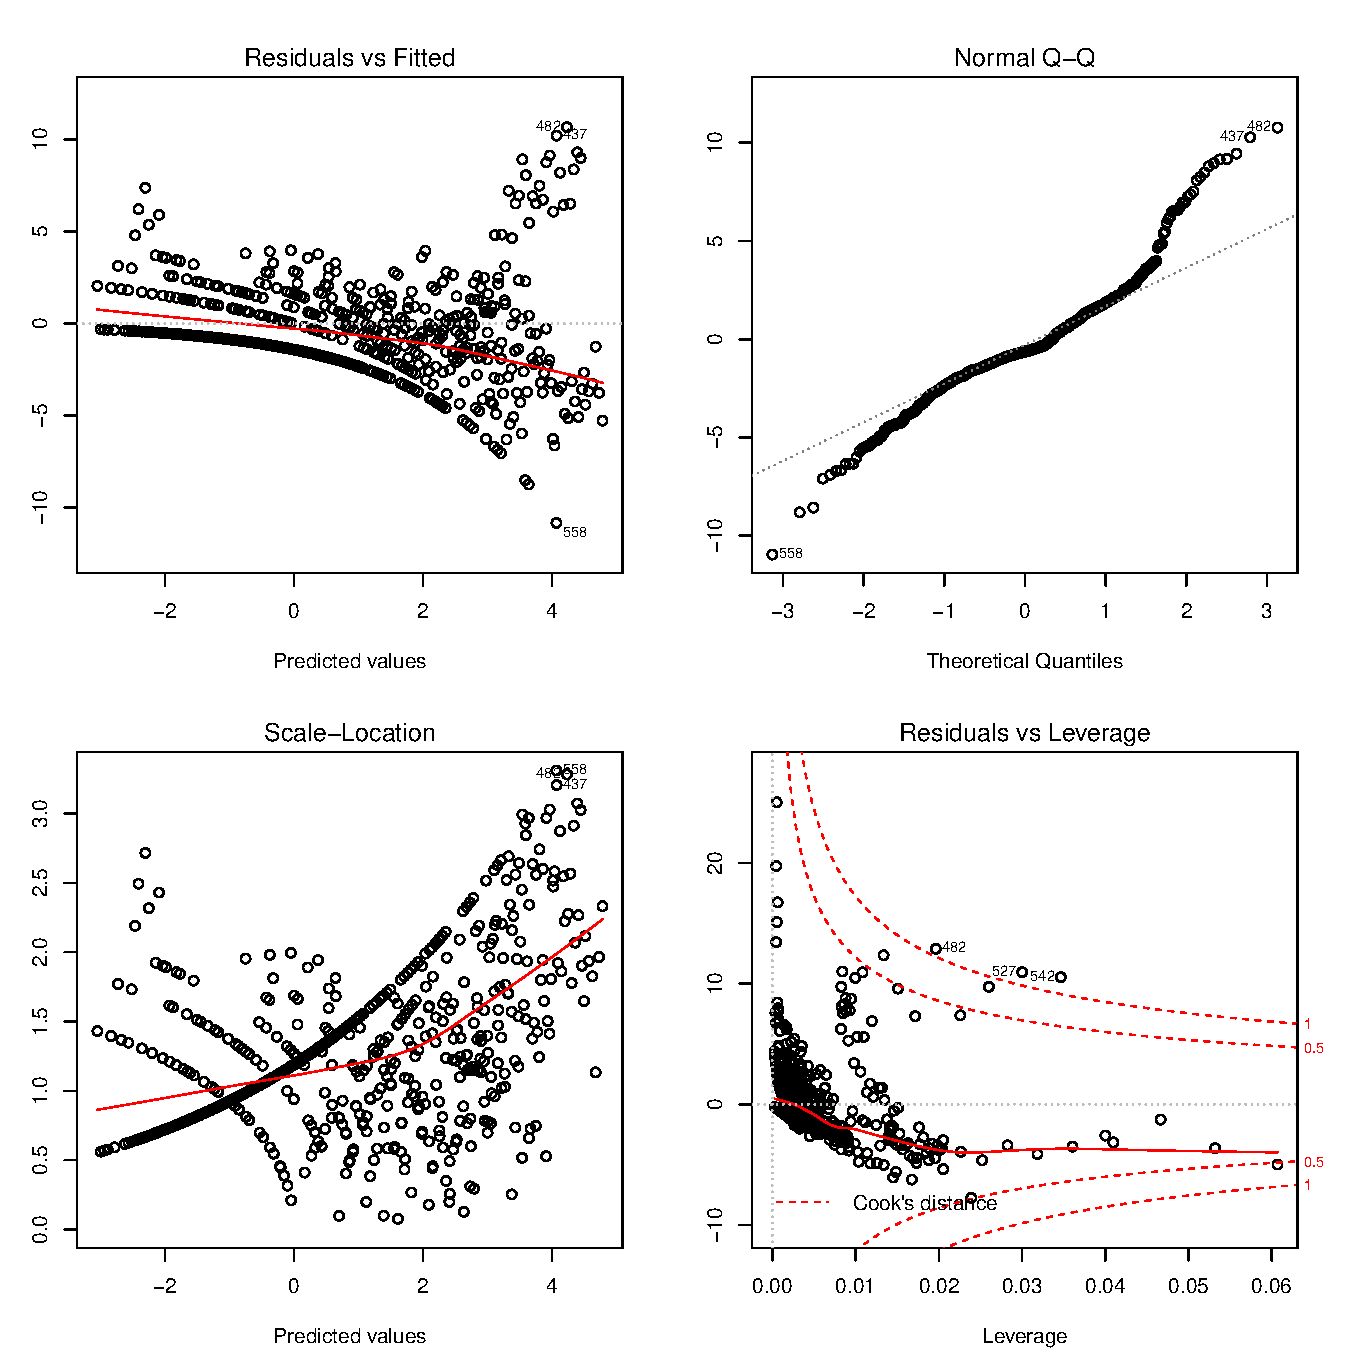
\includegraphics[width = 4in]{fig1.pdf}
	\caption{Diagnostic plots of Model 1.}
	\label{fig1}
\end{figure} 

\begin{figure}[h]
	\centering
	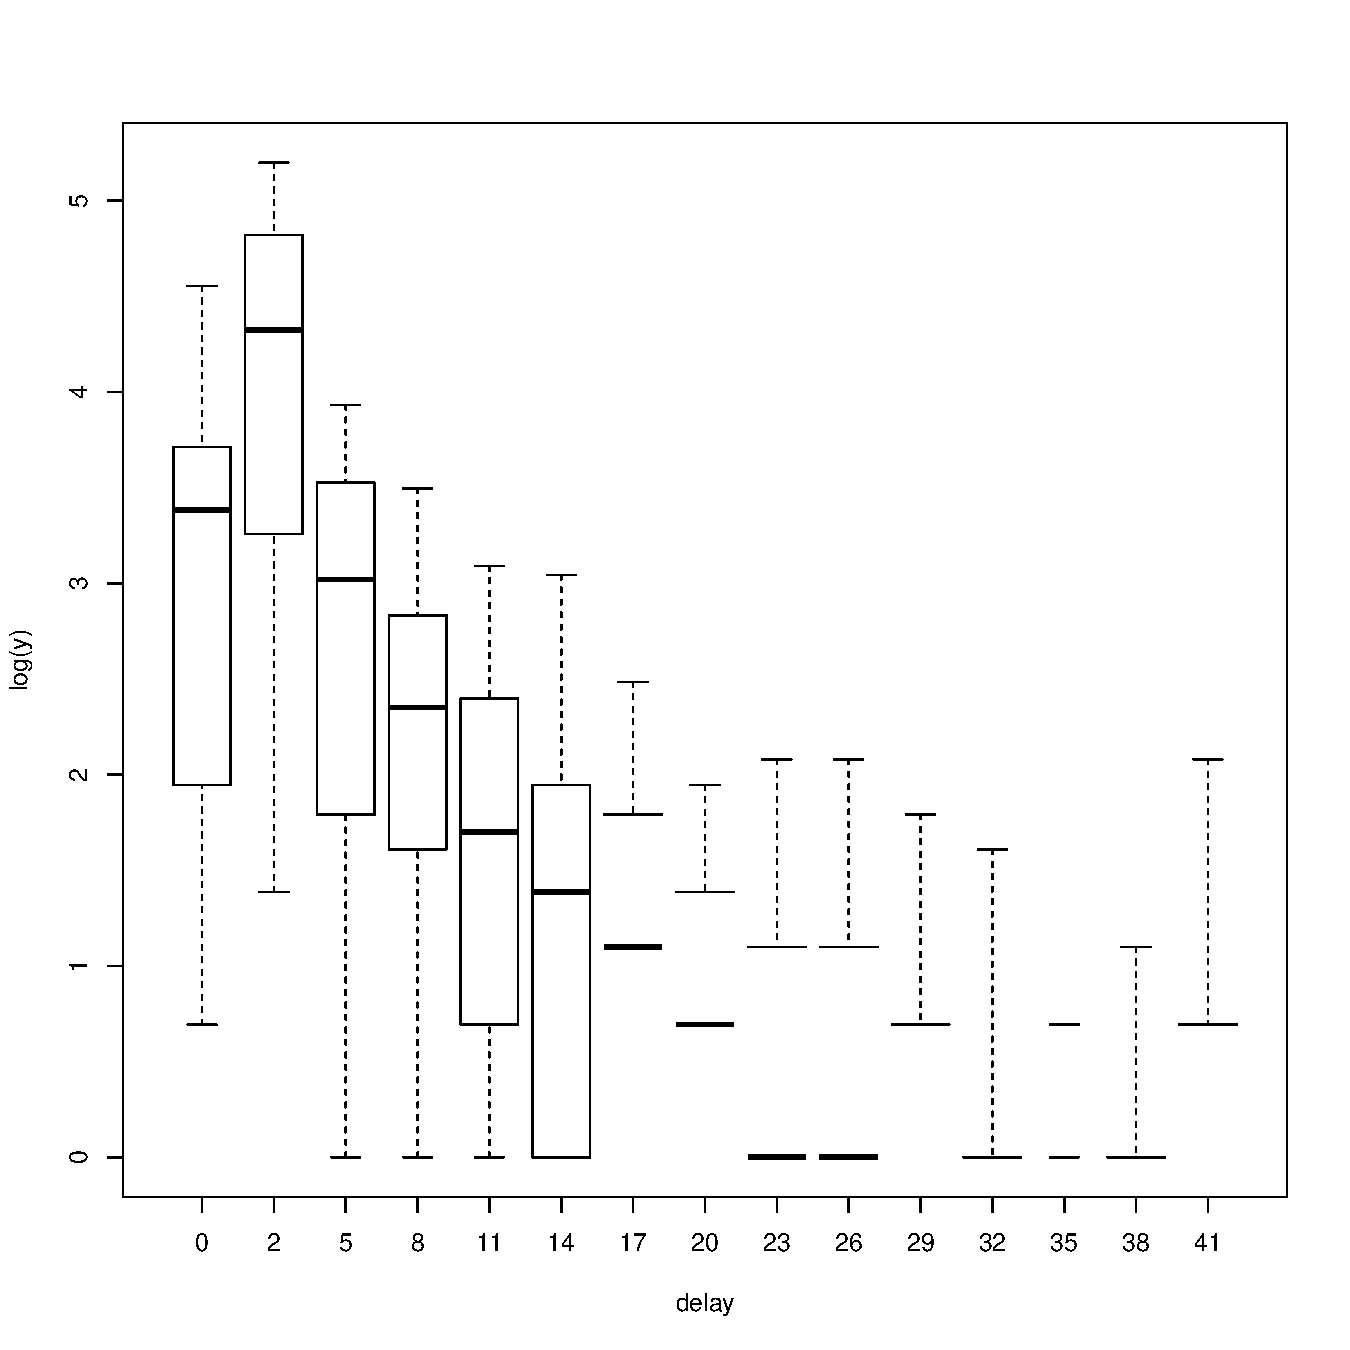
\includegraphics[width = 4in]{fig2.pdf}
	\caption{\texttt{log(y)} as a function of \texttt{delay}.}
	\label{fig2}
\end{figure} 

\begin{figure}[h]
	\centering
	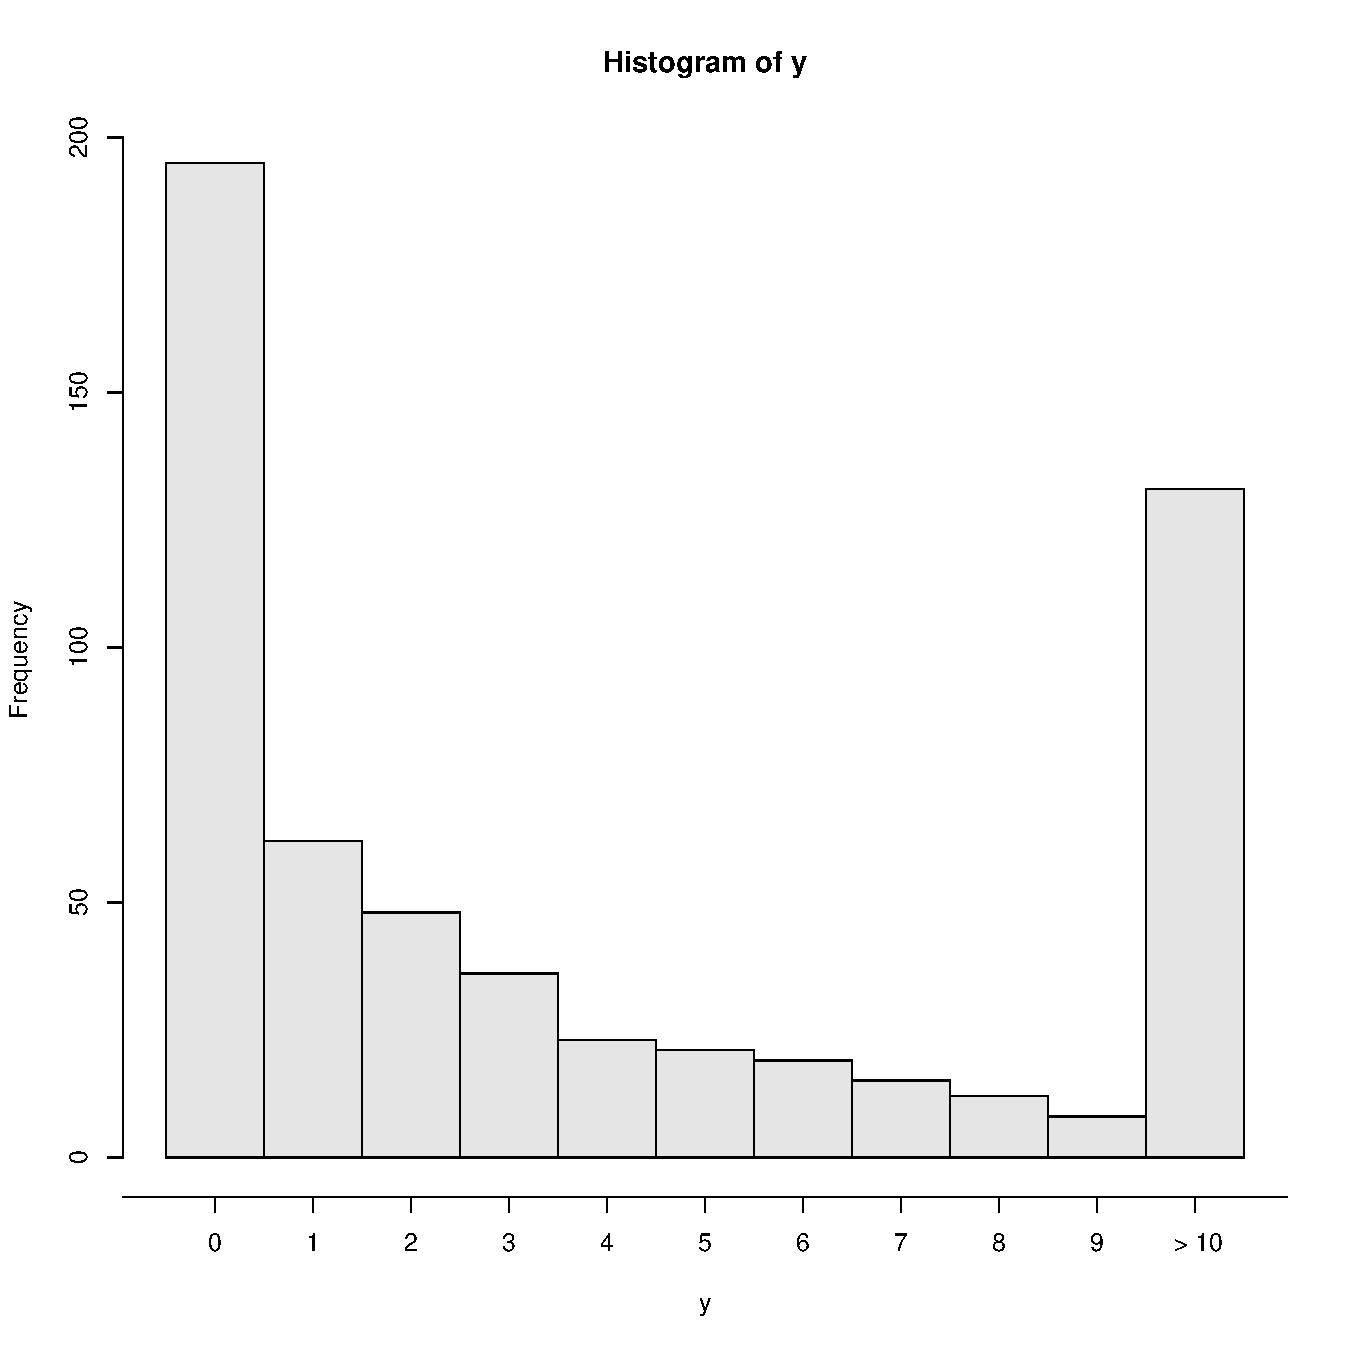
\includegraphics[width = 4.5in]{fig3.pdf}
	\caption{Distribution of \texttt{y}.}
	\label{fig2}
\end{figure} 


\question[4] Comment on Figure 1, 2 and 3. What potential problems in Model 1 could these figures suggest ? How would you address them ?
\begin{solution}
Model 1 doesn't seem to be a great fit : there are trends in the residual vs fitted plot and in the scale-location plots. Besides, there seems to be a few outliers, as suggested by the Residual vs leverage plot. Figure 2 suggests that a linear relation between $\log(E(\texttt{y}))$ and \texttt{delay} is irrelevant. Figure 3 suggests that there could be an excess of zeros in \texttt{y}. 

To deal with outlier, a robust GLM could be used; to deal with non-linearity of the \texttt{y} vs \texttt{delay} relationship, a GAM could be used ; and to deal with the excess of zeros, either a ZIP model or a Hurdle model could be used.
\end{solution}

\clearpage
 \fullwidth{We continued the analysis by fitting a GAM model, Model 3, presented in Output~\ref{out.gam} and Figure~\ref{fig4}.}

\begin{center}
	\begin{lstlisting}[caption = Model 3 (GAM). ,label=out.gam]
> fit_gam <- gam(y ~ s(time) + s(delay), data = aids, family = poisson)
> summary(fit_gam)

Family: poisson 
Link function: log 

Formula:
y ~ s(time) + s(delay)

Parametric coefficients:
Estimate Std. Error z value Pr(>|z|)    
(Intercept)  0.88146    0.03859   22.84   <2e-16 ***
---
Signif. codes:  0 '***' 0.001 '**' 0.01 '*' 0.05 '.' 0.1 ' ' 1 

Approximate significance of smooth terms:
edf Ref.df Chi.sq p-value    
s(time)  7.716  8.509   1541  <2e-16 ***
s(delay) 8.954  8.999   7440  <2e-16 ***
---
Signif. codes:  0 '***' 0.001 '**' 0.01 '*' 0.05 '.' 0.1 ' ' 1 

R-sq.(adj) =  0.867   Deviance explained = 87.2%
UBRE = 2.8257  Scale est. = 1         n = 570
AIC = 3578.037

> gam.check(fit_gam)

Method: UBRE   Optimizer: outer newton
full convergence after 9 iterations.
Gradient range [1.312875e-11,4.753834e-06]
(score 2.825708 & scale 1).
Hessian positive definite, eigenvalue range [0.0001600396,0.00211296].
Model rank =  19 / 19 

Basis dimension (k) checking results. Low p-value (k-index<1) may
indicate that k is too low, especially if edf is close to k'.

k'  edf k-index p-value    
s(time)  9.00 7.72    0.84  <2e-16 ***
s(delay) 9.00 8.95    0.42  <2e-16 ***
---
Signif. codes:  0 '***' 0.001 '**' 0.01 '*' 0.05 '.' 0.1 ' ' 1 
	\end{lstlisting}
\end{center} 

\begin{figure}[h]
	\centering
	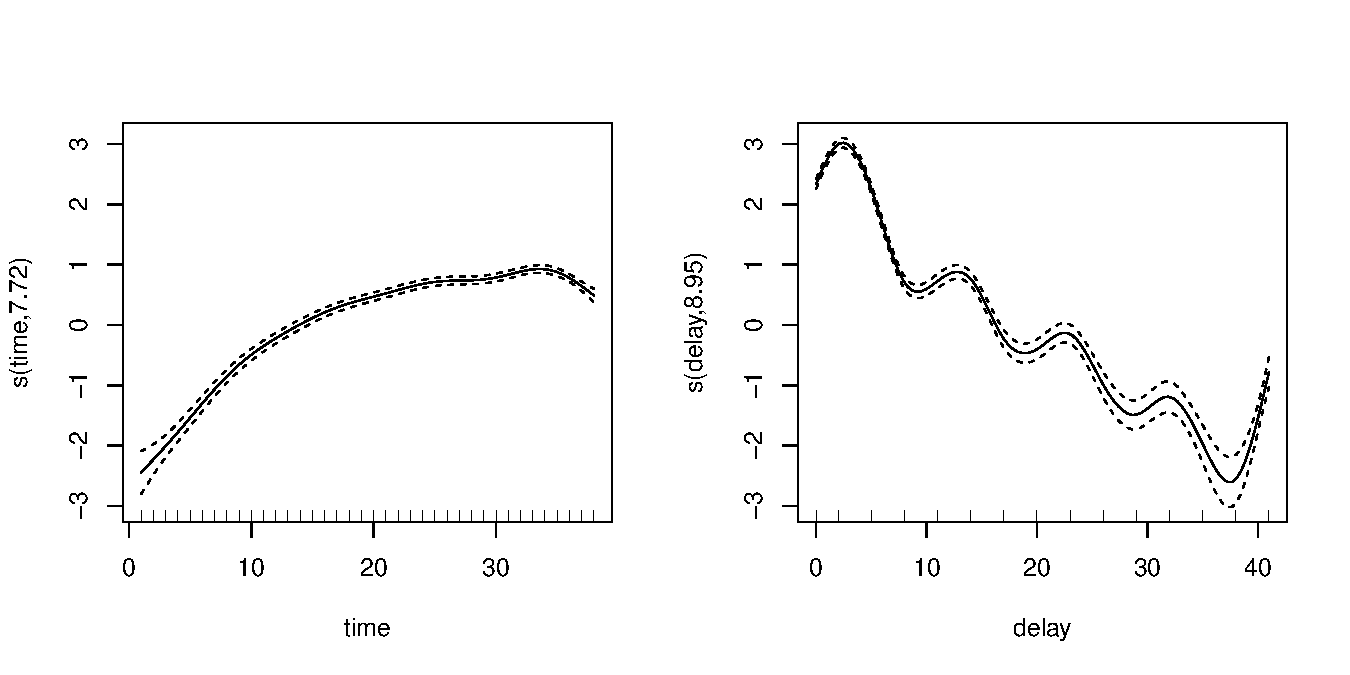
\includegraphics[width = 4.5in]{fig4.pdf}
	\caption{Fitted functions of the GAM Model~3.}
	\label{fig4}
\end{figure} 

\question[2] Can the AIC of the GAM model be compared to the GLM models' AIC ? 
\begin{solution}
	Yes, GLM is nested in GAMs.
\end{solution}
\question[2] Is GAM Model~3 more relevant than Model~1 ?
\begin{solution}
	Yes, we can see that it has the lowest AIC of all the other models considered so far. Figure~\ref{fig4} shows that the relationship between the response and the variables \texttt{time} and \texttt{delay} is significantly non linear.
\end{solution}
\question[2] Is the number of basis functions used for splines high enough ?
\begin{solution}
	We have to check in \texttt{gam.check(...)} if the p-values are low enough and if the k-index if significantly lower than the degrees of freedom. This is the case for the variable \texttt{time}, but for the variable \texttt{delay}, \texttt{k-index} is a bit close to \texttt{edf}, increasing the number of basis function for this variable could be necessary. 
\end{solution}

\clearpage
\fullwidth{We fitted another GAM model, Model~4, presented in Output~\ref{out.gam4} and Figure~\ref{fig5}.}

\begin{center}
	\begin{lstlisting}[caption = Model 4 (GAM). ,label=out.gam4]
	> fit_gam_quasi <- gam(y ~ s(time) + s(delay), data = aids, family = quasipoisson)
	> summary(fit_gam_quasi)
	
	Family: quasipoisson 
	Link function: log 
	
	Formula:
	y ~ s(time) + s(delay)
	
	Parametric coefficients:
	Estimate Std. Error t value Pr(>|t|)    
	(Intercept)  0.89611    0.06793   13.19   <2e-16 ***
	---
    Signif. codes:  0 '***' 0.001 '**' 0.01 '*' 0.05 '.' 0.1 ' ' 1 
	
	Approximate significance of smooth terms:
	edf Ref.df      F p-value    
	s(time)  5.651  6.764  70.28  <2e-16 ***
	s(delay) 8.827  8.987 255.94  <2e-16 ***
	---
	Signif. codes:  0 '***' 0.001 '**' 0.01 '*' 0.05 '.' 0.1 ' ' 1 
	
	R-sq.(adj) =  0.865   Deviance explained = 87.1%
	GCV = 3.9956  Scale est. = 3.2445    n = 570
	\end{lstlisting}
\end{center}

\begin{figure}[h]
		\centering
	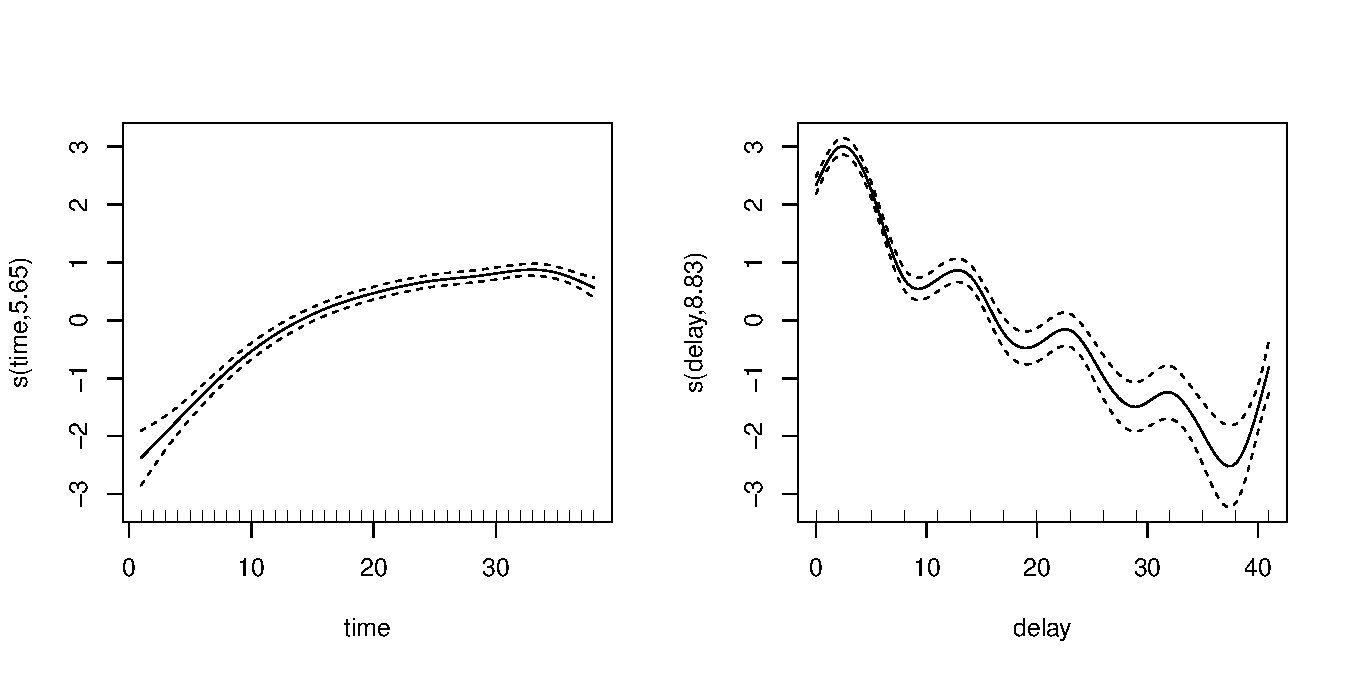
\includegraphics[width = 4.5in]{fig5.pdf}
	\caption{Fitted functions of the GAM Model~4.}
	\label{fig5}
\end{figure} 


\question[2] What is the difference between GAM Models~3 and~4 ? Explain.
\begin{solution}
Model 4 is a quasi-Poisson model. It allows the variance of the response to be different from its expectation (a constraint of the regular Poisson model). Estimates are the same for a Poisson and a quasi-Poisson model, but the variances of the estimates usually differ. This is what we can see by comparing Figures 4 and 5 : the curves are identical, but confidence intervals are wider for the quasi-Poisson model.
\end{solution}
\question[2] Could we compare the AIC of Model~3 with the AIC of Model~4 ?
\begin{solution}
No, because quasi-poisson models are note likelihood based (AIC is not defined).
\end{solution}


\clearpage
\fullwidth{We now consider the issue of excess of zeros.}

\question[2] Cite two models that deal with excess of zeros and describe the difference between them.
\begin{solution}
Zero Inflated Poisson model uses a latent Bernoulli variable, $B$. If $B = 0$, then the response is zero, otherwise, the response is distributed according to a Poisson distribution.

Hurdle model uses a Bernoulli variable, $B$. If $B = 0$, then the response is null, if $B = 1$, the response is distributed according to a truncated Poisson distribution. In this case the Bernoulli variable $B$ is not latent as we can observe it : it corresponds to the condition $Y = 0$.
\end{solution}

\fullwidth{Output~\ref{out.hurdle} shows a model, Model~5, accounting for excess of zeros.}

\begin{center}
	\begin{lstlisting}[caption = Model~5 (hurdle model). ,label=out.hurdle]
	> fit3_bin <- glm(I(y > 0) ~ delay + time, data = aids, family = binomial)
	> fit3_trunc <- glm(y ~ delay + time, data = aids, family = truncpoisson, 
	   subset = (y > 0))
	> fit3_bin
	
	Call:  glm(formula = I(y > 0) ~ delay + time, family = binomial, data = aids)
	
	Coefficients:
	(Intercept)        delay         time  
	3.39749     -0.10103     -0.02392  
	
	Degrees of Freedom: 569 Total (i.e. Null);  567 Residual
	Null Deviance:	    732.4 
	Residual Deviance: 571.6 	AIC: 577.6
	> fit3_trunc
	
	Call:  glm(formula = y ~ delay + time, family = truncpoisson, data = aids, 
	subset = (y > 0))
	
	Coefficients:
	(Intercept)        delay         time  
	2.54980     -0.12182      0.06106  
	
	Degrees of Freedom: 374 Total (i.e. Null);  372 Residual
	Null Deviance:	    11580 
	Residual Deviance: 2958 	AIC: 4098
	\end{lstlisting}
\end{center}
\question[2] According to Model~5, what is the probability that no case diagnosed at \texttt{time}$ = 11$ be reported to the Communicable Disease Surveillance Centre with a delay of 5 quarters ?
\begin{solution}
	\texttt{fit$\_$bin} models a Bernoulli variable indicating if \texttt{y} is zero or not. 
	$$\hat{\eta} = 3.397 - 0.101 \times 5 - 0.0239\times 11 \approx 2.63 .$$
	As the canonical link for binary model is logit, $\hat{p} = \frac{e^{2.63}}{1 + e^{2.63}} \approx 0.93$. As we model the probability that \texttt{y} is greater than $0$, the probability that \texttt{y} is equal to $0$ is $1 - 0.93 = 0.07$.	
\end{solution}
\question[2] Would it be relevant to compute the AIC of Model~5 by summing the AICs of \texttt{fit$\_$bin} and \texttt{fit$\_$trunc} presented in Output~\ref{out.hurdle}? Why ? Does Model~5 improve on Model~1 ?
\begin{solution}
	Yes, it would give the AIC of the Hurdle model. Indeed, the log-likelihood of the hurdle model splits into the log-likelihood of a binary model and the log-likelihood of a truncated Poisson model, each with their own sets of parameters.
	The AIC of Model 5 is thus $577.6 + 4098 = 4675.6$, which is lower than the AIC of Model 1.
\end{solution}


\question[2] Can the different models fitted previously answer the question "Is the delay between diagnosis and reporting to the Communicable Disease Surveillance Centre decreasing with time ?". If no, how would you proceed to answer it ? Share your reasoning, even if it is not conclusive.
\begin{solution}
	No they can't, as they don't consider any interaction between the variable \texttt{time} and \texttt{delay}. There are several ways to answer the question. 
	\begin{itemize}
		\item Consider a model with an interaction between \texttt{time} and \texttt{delay}. For instance \texttt{y} as a function of \texttt{delay + time + delay:time}. However, using GAM with such interaction could be delicate.
		\item Consider a model where the response reflects the delay rather than \texttt{y}. One could transform the data to have, for each value of \texttt{time} the proportion of \texttt{delay}s greater than some threshold among all cases diagnosed at that time. This proportion could then be used as the response in a binomial model.
	\end{itemize}
\end{solution}





\end{questions}

\clearpage
{\Large \textbf{Exercise 2} \hfill (24 points)}

\bigskip 

The Beta distribution is used to model proportions.  Assume that a random variable $Y$ follows a Beta distribution, with density

$$f(y; p,q) = \frac{\Gamma(p+q)}{\Gamma(p) \Gamma(q)}  y^{p-1} (1-y)^{q-1},$$
where $0<y<1$, $p>0$ and $q>0$. It holds that
$$E(Y) = \frac{p}{p+q},$$
and 
$$Var(Y) = \frac{pq}{(p+q)^2 (p+q+1)}.$$

\begin{questions}
\question[4] Consider the following transformation of parameters: $\mu = p/ (p+q)$ and
$\phi = p+q$. Rewrite the density $f$ as a function of $\mu$ and $\phi$ and give $E(Y)$ and $Var(Y)$ under this parametrization.

\begin{solution}
Because  $\mu = p/ (p+q)$ and $\phi = p+q$, we have $p = \mu \phi$ and $q = \phi - \mu \phi$, which gives
$$f(y; \mu, \phi) = \frac{\Gamma(\phi)}{\Gamma(\mu \phi) \Gamma ( \phi - \mu \phi)} y^{\mu \phi -1} (1-y)^{\phi - \mu \phi -1},$$
with $0<\mu<1$ and $\phi >0$.

We additionally have $E(Y) = \mu$ and 
$$Var(Y) = \mu(\phi - \phi \mu) \frac{1}{ \phi (\phi+1)} =  \frac{\mu(\phi - \phi \mu)}{\phi (\phi+1)} =  \frac{\mu(1 -  \mu)}{(\phi+1)}.$$

\end{solution}


\question[2]  Considering $\phi$ as a nuisance parameter, does the Beta distribution belongs to the one-parameter exponential family? 

\begin{solution}
We can write
\begin{eqnarray*}
\lefteqn{f(y; \mu, \phi) = }\\
& \exp \left( \ln(\gamma(\phi))  + (\mu \phi -1 ) \ln(y) + (\phi - \mu \phi -1) \ln(1-y) - \ln(\Gamma(\mu \phi)) - \ln(\Gamma(\phi - \mu \phi))  \right).
\end{eqnarray*}
 
By comparing this expression with the general form of the one-parameter exponential family (slides p.~52), we see that the Beta distribution does not belong to the exponential family.


\end{solution}


\question[2]  For each individual $i$ of a sample of size $n$, in addition to the
individual's response $y_i$, we have also measured a set of covariates $x_i$. We would like to use this information in a regression setting in a
GLM way. Suggest a possible model (in particular an appropriate link function), where the set of regression parameters will be denoted as $\beta$.

\begin{solution}

By analogy with the Bernoulli setting, and considering the role of the link function to guarantee that the estimated parameters lie in the admissible space of values, a logit link could be suggested, such that
$$\mbox{logit}\left( \frac{\mu}{1-\mu} \right) = x_i^T \beta.$$ 

The probit or complementary log-log link function could also be used. 

\end{solution}


\question[4] Write the log-likelihood associated with the model you have defined in 3. as a function of $\beta$ and $\phi$.

\begin{solution}
The likelihood function is

\begin{eqnarray*}
L(\mu,\phi; y_1, \ldots, n)  & = & \prod_{i=1}^n  \frac{\Gamma(\phi)}{\Gamma(\mu \phi) \Gamma ( \phi - \mu \phi)} y_i^{\mu \phi -1} (1-y_i)^{\phi - \mu \phi -1}\\
& = &  \frac{\Gamma^n(\phi)}{\Gamma^n(\mu \phi) \Gamma^n( \phi - \mu \phi)} \left( \prod_{i=1}^n y_i \right)^{\mu \phi -1} \left( \prod_{i=1}^n (1-y_i) \right)^{\phi - \mu \phi -1} 
\end{eqnarray*}
and therefore the log-likelihood as a function of $\mu$ and $\phi$ is

\begin{eqnarray*}
\lefteqn{l(\mu,\phi; y_1, \ldots, n)  = \ln \left(L(\mu,\phi; y_1, \ldots, n)  \right)} \\
& = & n \log(\Gamma(\phi)) - n \ln(\Gamma(\mu \phi)) -   n \ln(\Gamma( \phi - \mu \phi))) \\
&&+ (\mu \phi -1) \sum_{i=1}^n \ln(y_i) + (\phi - \mu \phi -1)  \sum_{i=1}^n \ln(1-y_i)
\end{eqnarray*}

The relationship imposed by the model is then used to replace $\mu$: 

$$\mu = \frac{\exp(x_i^T \beta)}{1+ \exp(x_i^T \beta)}.$$

\end{solution}

\fullwidth{We consider an application of the above model to the household food expenditure data from Griffiths et al. (1993). The dataset of samplesize 38 contains three variables: 
\begin{itemize}
\item \texttt{food}: food expenditure of the household
\item \texttt{income}: household income
\item \texttt{persons}: number of persons in the household
 \end{itemize}
 }


\clearpage
\fullwidth{Figure~\ref{foodexp} give a representation of the dataset and the fitted model is presented in Output~\ref{out.beta}.}

 
\begin{figure}[h]
	\centering
	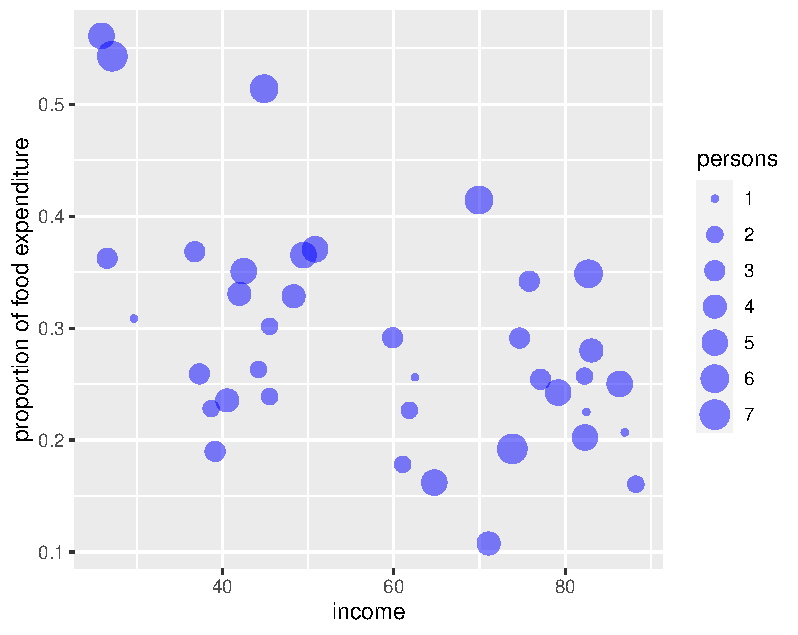
\includegraphics[width = 4.5in]{foodexp.pdf}
	\caption{Food expenditure data: proportion of household income spent on food as a function of household income. The size of the dots is proportional to the number of persons in the household.}
	\label{foodexp}
\end{figure} 

\begin{center}
	\begin{lstlisting}[caption = GLM Beta model with logit link. \\(Note: the \texttt{gam} function is used to fit the GLM model because is has a Beta family),label=out.beta]
> fit_beta <- gam(I(food/income) ~ income + persons,family=betar, data = FoodExpenditure)
> summary(fit_beta)

Family: Beta regression(33.032) 
Link function: logit 

Formula:
I(food/income) ~ income + persons

Parametric coefficients:
             Estimate Std. Error z value Pr(>|z|)    
(Intercept) -0.621147   0.231921  -2.678  0.00740 ** 
income      -0.012254   0.003142  -3.900 9.64e-05 ***
persons      0.118022   0.036595   3.225  0.00126 ** 
---
Signif. codes:  0 '***' 0.001 '**' 0.01 '*' 0.05 '.' 0.1 ' ' 1 

R-sq.(adj) =  0.438   Deviance explained = 41.6%
-REML =  -36.2  Scale est. = 1         n = 38
> logLik(fit_beta)
'log Lik.' 45.28002 (df=....)

	\end{lstlisting}
\end{center}

\question[2]  What is the effect of increasing the number of persons in the household on the expected proportion of food expenditure?

\begin{solution}
The sign of the coefficient of \texttt{persons} is positive, therefore implying that if the number of persons increases, the proportion of food expenditures increases as well (for constant income), which matches the intuition.
\end{solution}

\question[4] A household with 4 persons and an income equal to 60 is planning to welcome an Ukrainian refugee. Quantify the expected proportion of food expenditure change.

\begin{solution}
The logit link is used, therefore we can estimate the proportion of food expenditures by
$$\hat{\mu} = \frac{\exp \left(  -0.621147  -0.012254 * \texttt{income} +  0.118022 * \texttt{persons} \right)}{1 + \exp \left(  -0.621147  -0.012254 *\texttt{income} +  0.118022 * \texttt{persons} \right)}.$$

If \texttt{income} = 60 and \texttt{persons} = 4, we have  $\hat{\mu} = 0.2923$, whereas if \texttt{income} = 60 and \texttt{persons}= 5, we have $\hat{\mu} = 0.3173$. The proportion of food expenditures is expected to increase from $29.23\%$ to $31.73\%$.

\end{solution}




\question[2] Compute the AIC of the Beta model in Output~\ref{out.beta}.
\begin{solution}
AIC = -2*45.28 + 2 *4 =  -82.56
\end{solution}

\fullwidth{We also fitted  a GAM model. Output~\ref{out.beta.gam} gives the details of the fitted model and Figure~\ref{foodexpGAM} depicts the nonparametric fitted functions.}


\begin{center}
	\begin{lstlisting}[caption = GAM Beta model with logit link. ,label=out.beta.gam]
> fit_beta_gam <- gam(I(food/income) ~ s(income) + s(persons,k=7), family=betar, 
   data = FoodExpenditure)
   
> summary(fit_beta_gam)

Family: Beta regression(34.779) 
Link function: logit 

Formula:
I(food/income) ~ s(income) + s(persons, k = 7)

Parametric coefficients:
            Estimate Std. Error z value Pr(>|z|)    
(Intercept) -0.91450    0.06034  -15.15   <2e-16 ***
---
Signif. codes:  0 '***' 0.001 '**' 0.01 '*' 0.05 '.' 0.1 ' ' 1 

Approximate significance of smooth terms:
             edf Ref.df Chi.sq  p-value    
s(income)  1.851  2.312  17.94 0.000257 ***
s(persons) 1.000  1.000  10.54 0.001168 ** 
---
Signif. codes:  0 '***' 0.001 '**' 0.01 '*' 0.05 '.' 0.1 ' ' 1 

R-sq.(adj) =  0.467   Deviance explained =   46%
-REML = -40.009  Scale est. = 1         n = 38

> AIC(fit_beta_gam)
[1] -82.79725
	
	\end{lstlisting}
\end{center}

\begin{figure}[h]
	\centering
	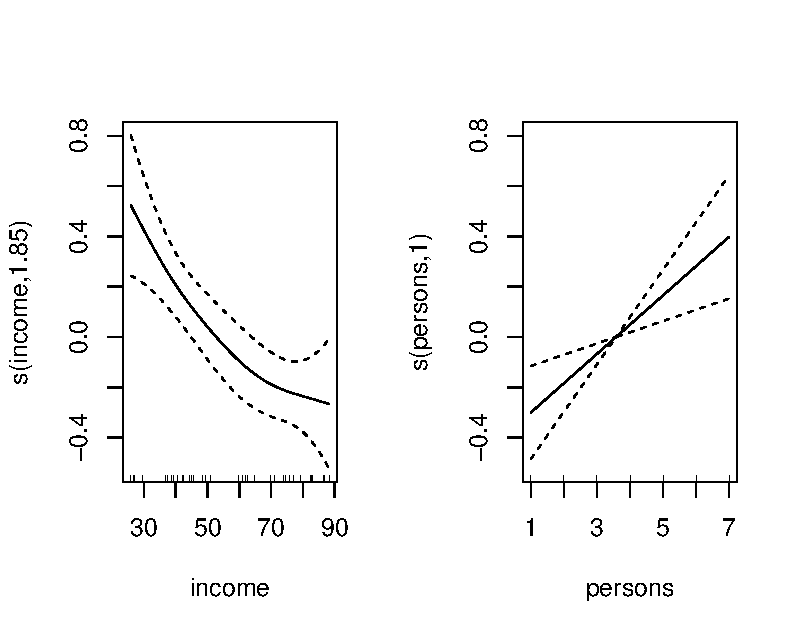
\includegraphics[width = 5in]{foodexpGAM.pdf}
	\caption{Fitted functions of the GAM model.}
	\label{foodexpGAM}
\end{figure} 

\question[2]  What is the argument $\texttt{k}$ in \texttt{s(persons, k = 7)} in Output~\ref{out.beta.gam}? Why has it been set to~7?


\begin{solution}
$\texttt{k}$ is the number of basis functions used in the spline fit. It cannot be larger than 7  because the variable \texttt{persons} only takes 7 distincts values.

\end{solution}

\question[2] Are the nonparametric fits worth the trouble?

\begin{solution}
The fitted function for \texttt{persons} is linear and the fitted function for \texttt{income} is almost linear. The AIC does not change much, but the percentage of deviance explained increases with the GAM model. Both models seem to be equally good. 

\end{solution}

\end{questions}
\clearpage

\begin{table}
	\begin{center}
	\begin{tabular}{ |c|c|c|c|c|c| } 
		\hline
		df & 0.75 & 0.90 & 0.95 & 0.975 & 0.99\\
		\hline
	1 & 1.323  & 2.706 & 3.841 & 5.024 & 6.635 \\
	40 & 45.62 & 51.81 & 55.76 & 59.34 & 63.69 \\
	80 & 88.13 &  96.58 & 101.9 & 106.6 & 112.3 \\
	120 & 130.1 & 140.2 & 146.6 & 152.2 & 159.0 \\
	160 & 171.7 & 183.3 & 190.5 & 196.9 & 204.5 \\
	200 & 213.1 & 226.0 & 234.0 & 241.1 & 249.4 \\
	240 & 254.4 & 268.5 & 277.1 & 284.8 & 293.9 \\
	280 & 295.6 & 310.7 & 320.0 & 328.2 & 338.0 \\
	320 & 336.7 & 352.8 & 362.7 & 371.4 & 381.8 \\
	360 & 377.7 & 394.8 & 405.2 & 414.5 & 425.3 \\
	400 & 418.7 & 436.6 & 447.6 & 457.3 & 468.7 \\
	440 & 459.6 & 478.4 & 489.9 & 500.0 & 511.9 \\
	480 & 500.5 & 520.1 & 532.1 & 542.6 & 555.0 \\
	520 & 541.4 & 561.7 & 574.2 & 585.1 & 597.9 \\
	560 & 582.2 & 603.3 & 616.2 & 627.5 & 640.8 \\
	600 & 623.0 & 644.8 & 658.1 & 669.8 & 683.5 \\
	640 & 663.8 & 686.3 & 700.0 & 712.0 & 726.2 \\
	680 & 704.5 & 727.7 & 741.8 & 754.2 & 768.7 \\
	720 & 745.2 & 769.0 & 783.5 & 796.3 & 811.2 \\
	760 & 785.9 & 810.4 & 825.2 & 838.3 & 853.6 \\
			\hline
	\end{tabular}
\caption{Quantiles of a $\chi^2$ distribution, depending on the degrees of freedom df, for probabilities $0.75, 0.9, 0.95, 0.975$ and $0.99$}
\end{center}
\end{table}


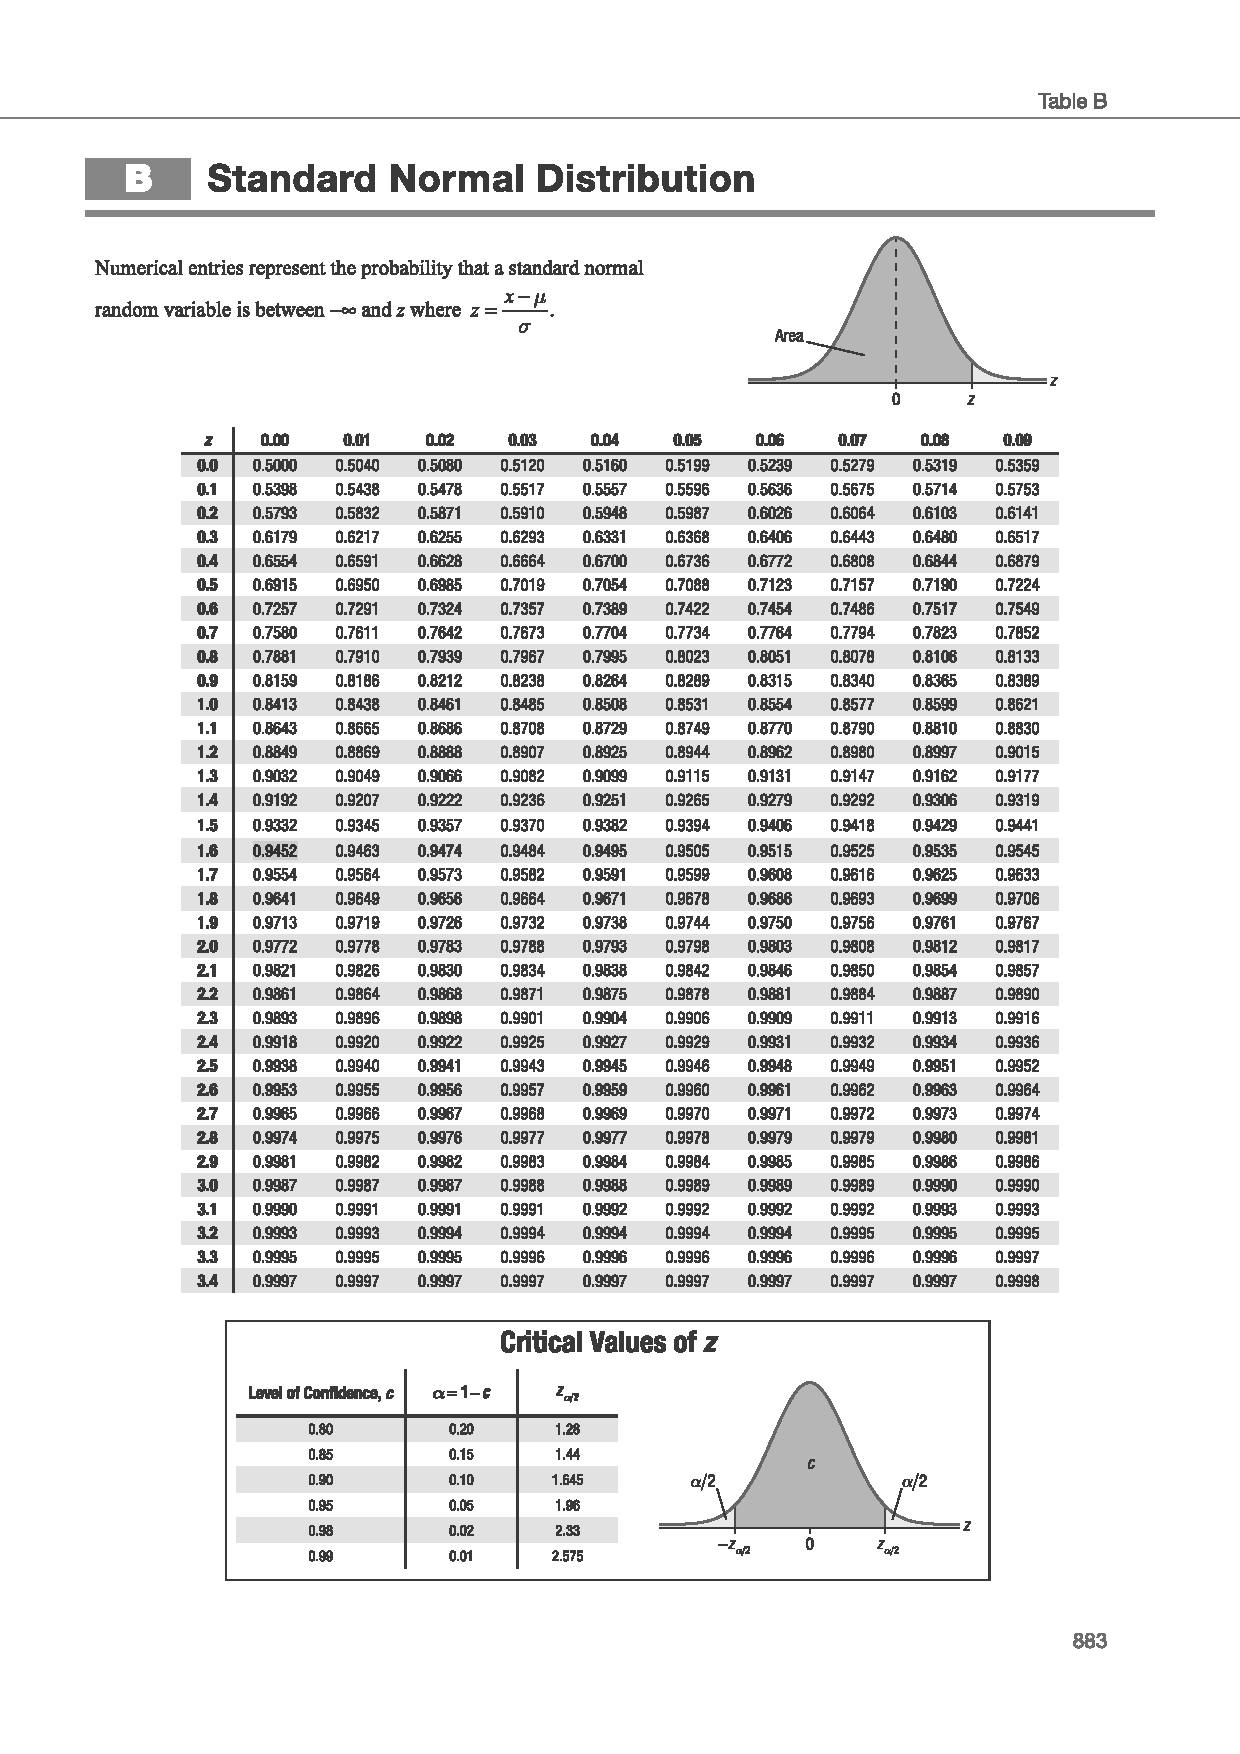
\includepdf[pages=-]{tables_norm.pdf}


\end{document}

